\documentclass[11pt,a4paper]{article}
\usepackage{pgf}
\usepackage{tikz}
\usepackage{multirow}
\usepackage{url}
\usepackage{hyperref}
\usepackage{graphicx}

\setlength{\oddsidemargin}{0in}
\setlength{\evensidemargin}{0in}
\setlength{\headheight}{12pt}
\setlength{\headsep}{60pt}
\setlength{\topmargin}{-90pt}
\setlength{\textwidth}{6.5in}
\setlength{\textheight}{10in}

\begin{document}

\title{On Capabilities Feature of Amoeba}
\author{Attique Dawood}
\maketitle

\section{Introduction to Amoeba Operating System}

Amoeba is a distributed operating system developed at Vrije Universiteit, Amsterdam. The chief designer was Andrew S. Tanenbaum. It was designed to be transparent with user not having to worry about underlying hardware, like number of processors. The user only sees interacting with a single powerful system~\cite{distributed-systems-book}.

\begin{figure}[here]
%\centerline{\includegraphics[]{GPGPU}}
\centering
\begin{tikzpicture}
	\draw[very thick] (0cm, 0cm) rectangle (2.1cm, 2cm);
	\foreach \x in {0.1cm,0.6cm,1.1cm, 1.6cm}
		\filldraw[gray, thick] (\x, 0.9cm) rectangle (\x+0.4cm, 1.9cm);
	\coordinate [label=above:CPU] (CPU) at (1.05cm,0.2cm);
	\coordinate [label=below:CPU with multiple cores] (Multi Core CPU) at (1.05cm,-0.2cm);
	
	\draw[very thick, <->, >=stealth] (2.5cm, 1cm) -- (3.1cm, 1cm);
	
	\draw[very thick] (3.5cm, -1cm) rectangle (7.6cm, 3cm);
		\foreach \x in {3.6cm,4cm,4.4cm,4.8cm,5.2cm,5.6cm,6cm,6.4cm,6.8cm,7.2cm}
			\foreach \y in {0.2cm,0.6cm,1cm,1.4cm,1.8cm,2.2cm,2.6cm}
				\filldraw (\x, \y) rectangle (\x+0.3cm, \y+.3cm);
	\coordinate [label=above:GPU] (GPU) at (5.55cm,-0.7cm);
	\coordinate [label=below:GPU with lots of cores] (Multi Core GPU) at (5.55cm,-1.3cm);		
\end{tikzpicture}
\caption{GPGPU Computing.}
\label{nVidiaGPGPUfig}
\end{figure}

\section{Project Overview}
A central server will be connected to multiple computers (hosts) with GPUs (devices). Clients will connect to the server through a secure channel. Clients will request computational resource(s) and upload their code. The server will look for any free devices and make allocation as necessary. Client code will compile and run on a free device and output will be returned. In case of compilation errors client will be notified.

\begin{figure}[here]
%\centerline{\includegraphics[]{GPGPU}}
\centering
\begin{tikzpicture}
	\draw[very thick] (6cm, 4cm) rectangle (8cm, 5cm);
	\coordinate [label=above:{\bfseries Server}] (Server) at (7cm,4.25cm);
	
	\draw[thick,<->, >=stealth] (8.1cm,4.5cm) -- (10.8cm, 5.8cm);
	\draw[very thick] (11cm, 5.3cm) rectangle (13cm, 6.3cm);
	\coordinate [label=above:{\bfseries GPU}] (GPU) at (12cm,5.55cm);
	
	\draw[thick,<->, >=stealth] (8.1cm,4.5cm) -- (10.8cm, 4.5cm);
	\draw[very thick] (11cm, 4cm) rectangle (13cm, 5cm);
	\coordinate [label=above:{\bfseries GPU}] (GPU) at (12cm,4.25cm);
	
	\draw[thick,<->, >=stealth] (5.9cm,4.5cm) -- (3.2cm, 5.8cm);
	\draw[very thick] (1cm, 4cm) rectangle (3cm, 5cm);
	\coordinate [label=above:{\bfseries Client}] (Client) at (2cm,4.25cm);
	
	\draw[thick,<->, >=stealth] (5.9cm,4.5cm) -- (3.2cm, 4.5cm);
	\draw[very thick] (1cm, 5.3cm) rectangle (3cm, 6.3cm);
	\coordinate [label=above:{\bfseries Client}] (Client) at (2cm,5.55cm);
	
	\draw[very thick,dotted] (2cm, 2.7cm) -- (2cm, 3.8cm);
	
	\draw[thick,<->, >=stealth] (5.9cm,4.5cm) -- (3.2cm, 2cm);
	\draw[very thick] (1cm, 1.5cm) rectangle (3cm, 2.5cm);
	\coordinate [label=above:{\bfseries Client}] (Client) at (2cm,1.75cm);

\end{tikzpicture}
\caption{Project Overview.}
\label{ProjectOverview}
\end{figure}

\section{Project Phases}

This project is divided into three phases:

\subsection{Phase I: Network Programming}
The first phase is to implement the client--server at application layer. Server should be able to handle multiple clients at a time. It should also be able to support multiple simultaneous connections both to clients and GPU hosts. Server will maintain a dynamic list of computational resources available and those which are in use.

\subsection{Phase II: GPU Programming}
The hosts with GPUs should be able to receive client code and compile it on the fly. In case of errors, appropriate error messages must be relayed to client through server. A mini--compiler can be implemented at the host which can convert conventional loop--based code into appropriate kernel code to be run on GPU. 

Another aspect is multi--GPU computing where a number of GPUs are available to the client. Client can request multiple GPUs in order to speed up the computation. In hybrid multi--GPU context, multiple GPUs running different APIs such as CUDA and OPENCL can be combined to work on a single problem. Synchronization is an important issue in such a scenario.

\subsection{Phase III: Security}
All communication from clients to server to GPU hosts must be secure. Network traffic must be encrypted to keep out eavesdropping. PGP can be a good choice of security. Clients can be assigned usernames/passwords beforehand to only allow trusted access. PGP on top of it can provide additional layer of security if any password(s) are compromised.

\section{Project Timeline}

Major focus will be on the network programming part. Rest of the functionality will depend on robustness and features of client--server application.

Following table provides a tentative timeline for this project:

\begin{table}[h]
\begin{center}
\vspace{0.3cm}
	\begin{tabular}{llp{10cm}}
	\hline \hline
		\textbf{Week} \rule{0pt}{2.6ex} & \textbf{Duration} & \multicolumn{1}{c}{\textbf{Tasks}}\\
		\hline
		2 \rule{0pt}{2.6ex} & 1 week & Set and install network programming APIs on PCs\\
		3 & 1 week & Implement a simple client--server application for handling multiple clients\\
		4-6 & 3 weeks & Implement core features of network programming\\
		7-8 & 2 weeks & Set up GPUs and install GPU programming APIs\\
		9-10 & 2 weeks & Provide GPU programming interface to clients through server over network\\
		11-12 & 2 weeks & Refinements\\
		13-15 & 3 weeks & Encrytion of network traffic and additional security features like PGP\\
	\hline \hline
	\end{tabular}
\end{center}
\label{TimelineTable}
\caption{Project timeline.}
\end{table}
\nocite{*}
\bibliographystyle{plain}
\bibliography{Amoebaref}

%\begin{thebibliography}{99}


%\bibitem{amoeba-sourceforge}
%http://fsd-amoeba.sourceforge.net/amoeba.html

%\bibitem{nVidiaGPGPU}
%George Coulouris, Jean Dollimore \& Tim Kindberg,
% ``Distributed Systems''


%\bibitem{AMDATiGPGPU}
%http://www.amd.com/us/products/technologies/stream-technolo %gy/opencl/pages/gpgpu-history.aspx

%\end{thebibliography}

\end{document}




